\subsubsection{Minuta de reunião (01-Julho-2015)}

\begin{tabbing}
  Local \= xxx \kill
  Local \> : LEAD \\
  Data  \> : 01 de Julho de 2015 \\
  Hora  \> : 13:00
\end{tabbing}

%---------------------------------------------------------------------
\participantes{
  \elael,
  \alana,
  \gabriel,
  \julia,
  \ramon,
  \renan.
}

\textbf{Aprovação da minuta}

\textbf{Update semanal do Projeto EMMA}

\textbf{Considerações Gerais EMMA:}
  \begin{itemize}
    \item Contratações previstas: 1 engenheiro de software, 1 engenheiro de
    eletrônica e um aluno de mestrado de controle.
    \item Primeiro Objetivo do quadrimestre: definir a solução detalhada.
    Análise de riscos e benefícios.
    \item Segundo Objetivo do Quadrimentre: Determinar a relação de posição do
    braço robótico e do ambiente.
    \item Terceiro Objetivo do Quadrimentre: elaboração de tarefas do robô em
    preparo para arquitetura de interface.
  \end{itemize}
  
  
\textbf{\renan.} 
	\begin{itemize}
		\item \textbf{Tarefas concluídas:}
			\begin{itemize}    
				\item SOTA.
			\end{itemize}
		
		\item \textbf{Novas tarefas:}
			\begin{itemize} 
				\item Detalhes do acesso do robô na escotilha inferior.
				\item Apresentação.
			\end{itemize}
	\end{itemize}
		
\textbf{\elael.} 
	\begin{itemize}
		\item \textbf{Tarefas concluídas:}
			\begin{itemize}    
				\item SOTA
			\end{itemize}
		
		\item \textbf{Novas tarefas:}
			\begin{itemize} 
				\item Pesquisar sensores. Localização e Octomap para ajudar no processo de
				de calibração do braço Robótico.
				\item Mapeamento de tarefas do robô para interface de usuário.
			\end{itemize}
	\end{itemize}
					
			
   \textbf{\gabriel.} 
	\begin{itemize}
		\item \textbf{Tarefas concluídas:}
			\begin{itemize}    
				\item SOTA.
			\end{itemize}
		
		\item \textbf{Novas tarefas:}
			\begin{itemize} 
			    \item Procurar OpenSource para auxiliar no processo de calibração do
			    braço robótico.
				\item Mapeamento de tarefas do robô para interface de usuário.
			\end{itemize}
	\end{itemize}

			
		
   \textbf{\estevão.} 
	\begin{itemize}
		\item \textbf{Tarefas concluídas:}
			\begin{itemize}    
				\item SOTA.
			\end{itemize}
		
		\item \textbf{Novas tarefas:}
			\begin{itemize} 
			    \item Definir conceito da base para suporte de manipulador na entrada da
			    escotilha inferior.
			\end{itemize}
	\end{itemize}
	
		
   \textbf{\estevão.} 
	\begin{itemize}
		\item \textbf{Tarefas concluídas:}
			\begin{itemize}    
				\item Apresentação
			\end{itemize}
		
		\item \textbf{Novas tarefas:}
			\begin{itemize} 
			    \item Estudo das tarefas do robô e seu mapeamento para a construção da
			    interface de usuário.
			\end{itemize}
	\end{itemize}

			



\textbf{Agenda para a próxima reunião:}
  \begin{itemize}
    \item Resultado de pesquisas individuais.
    \item Novas tarefas \& recomendações.
  \end{itemize}


\vspace{5mm}%
\parbox[t]{70mm}{
  Aprovado por: \\[5mm]
  \centering
  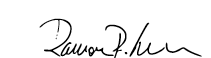
\includegraphics[width=65mm]{figs/logo/assinatura-ramon.png} \\[-4mm]
  \rule[2mm]{70mm}{0.1mm} \\
  \ramon \\[1mm]
  Coordenador do Projeto \\
}

%---------------------------------------------------------------------
\fim